%!TEX root = ../DissertationDefensePresentation.tex

%%--------------------------------------------------------------------------------------------

%\subsection{Limits}

%%--------------------------------------------------------------------------------------------
\begin{frame}
	\frametitle{Results}
	\vspace*{-0.24cm}
	%\begin{alertblock}{}
		\begin{myfancyblock}
    		\node[anchor=south west,inner sep=0] (image) at (0,0) {%
    		   \hspace*{0.15cm}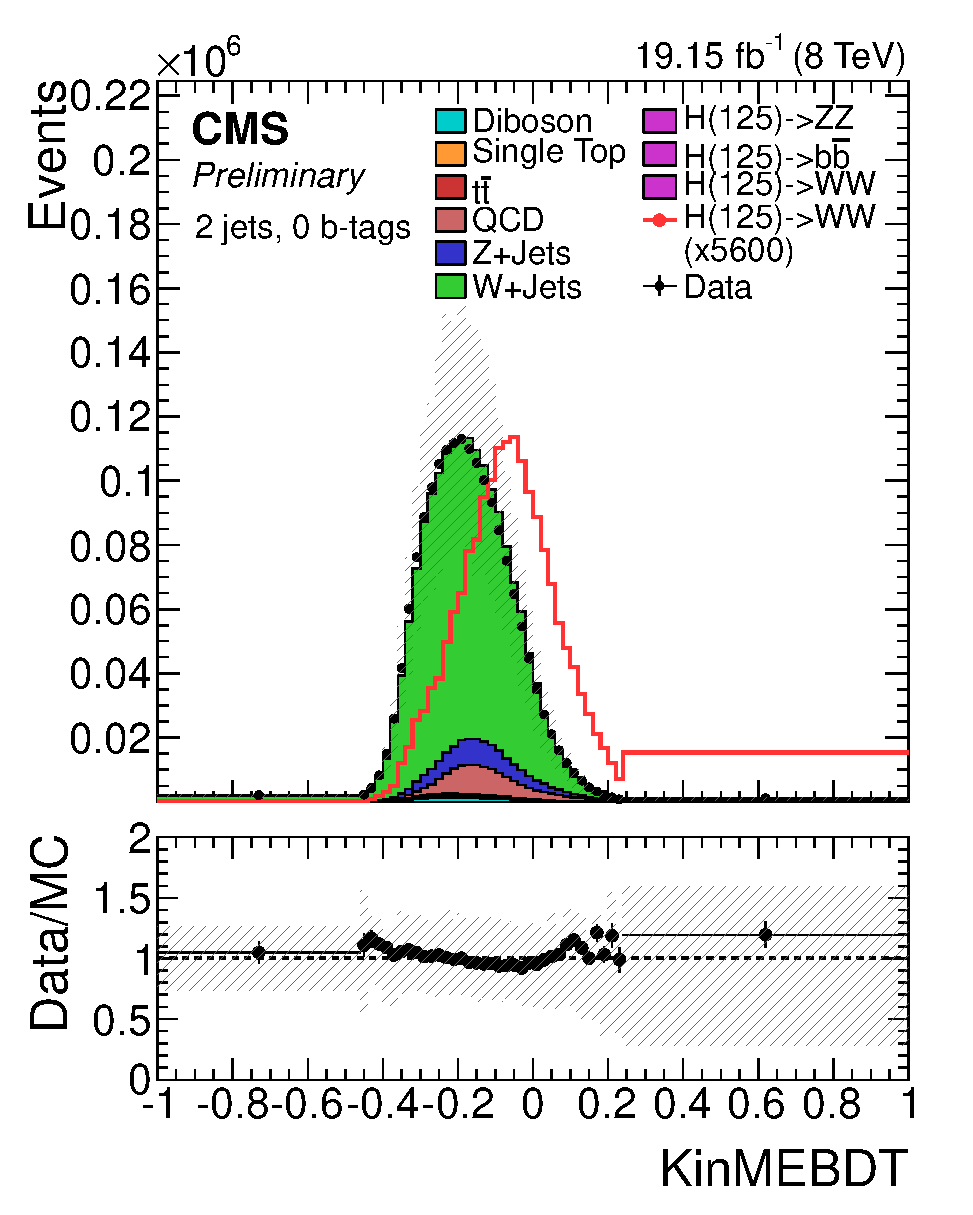
\includegraphics[width=0.26\textwidth]{\figpath/KinMEBDT_jets2_electron.eps}%
    		   \hspace*{0.15cm}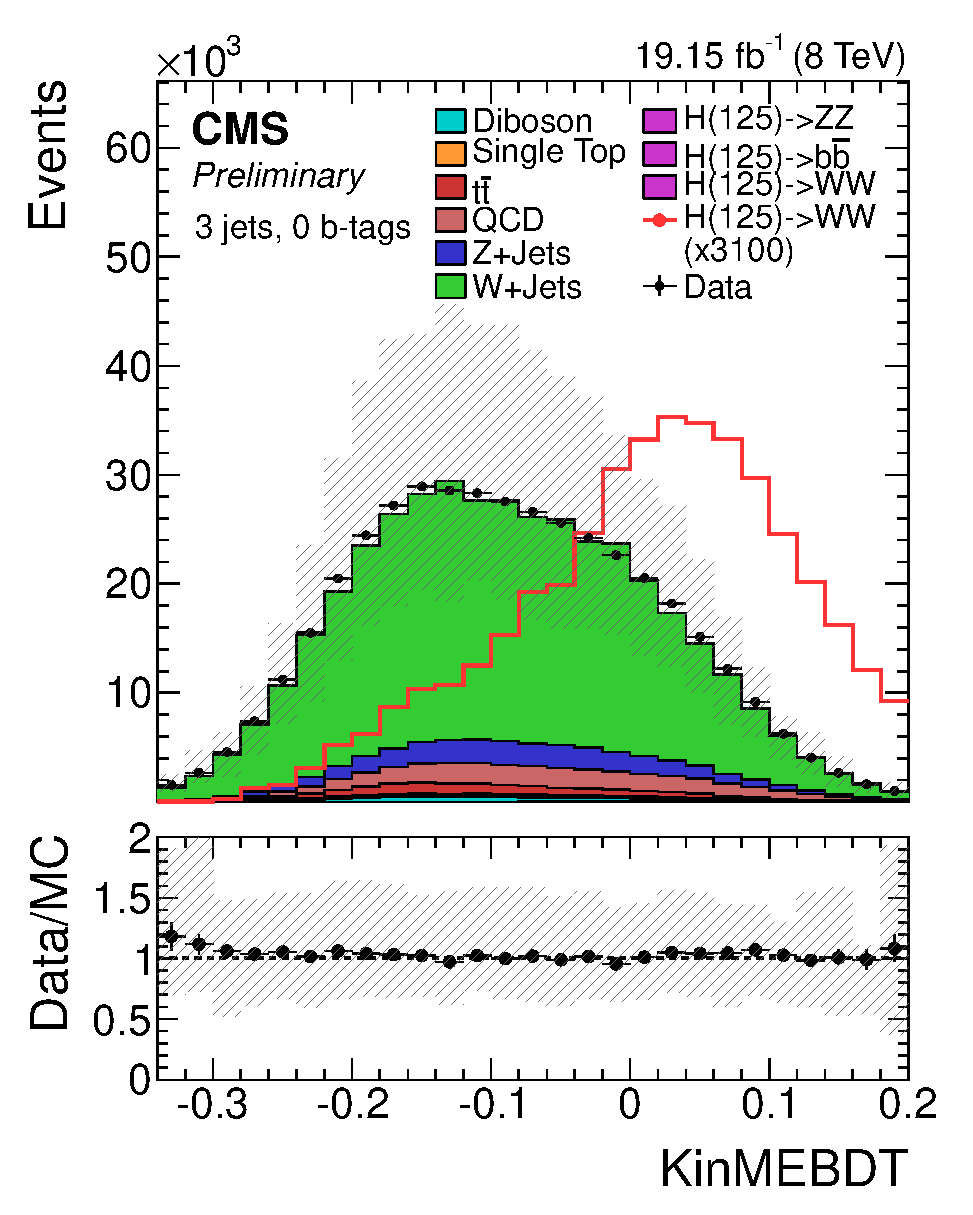
\includegraphics[width=0.26\textwidth]{\figpath/KinMEBDT_jets3_electron.eps}%
    		   \hspace*{0.15cm}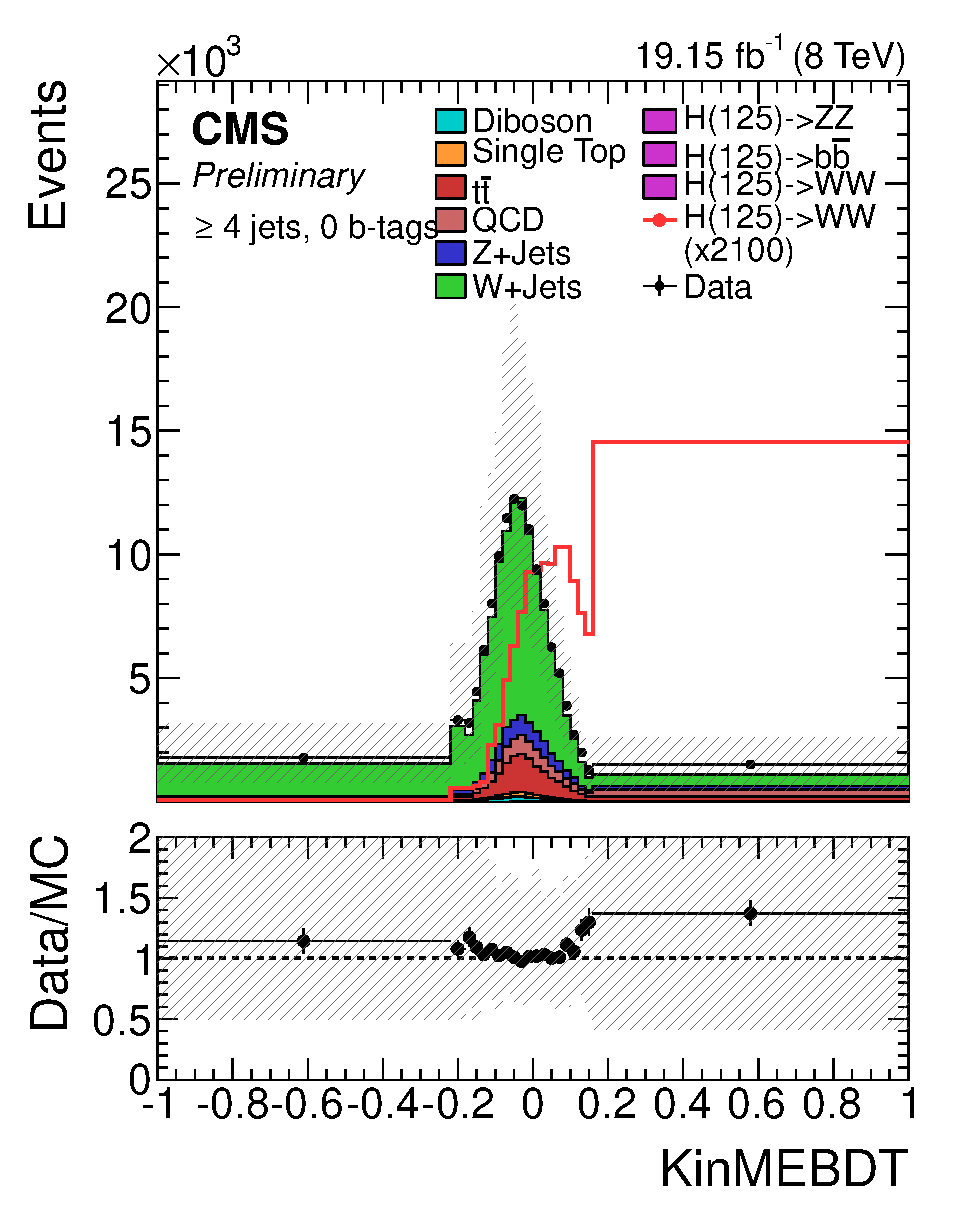
\includegraphics[width=0.26\textwidth]{\figpath/KinMEBDT_jets4_electron.eps}%
    		};
    		\node[anchor=south west,inner sep=0] (image2) at (0,-4.1) {%
    		   \hspace*{0.15cm}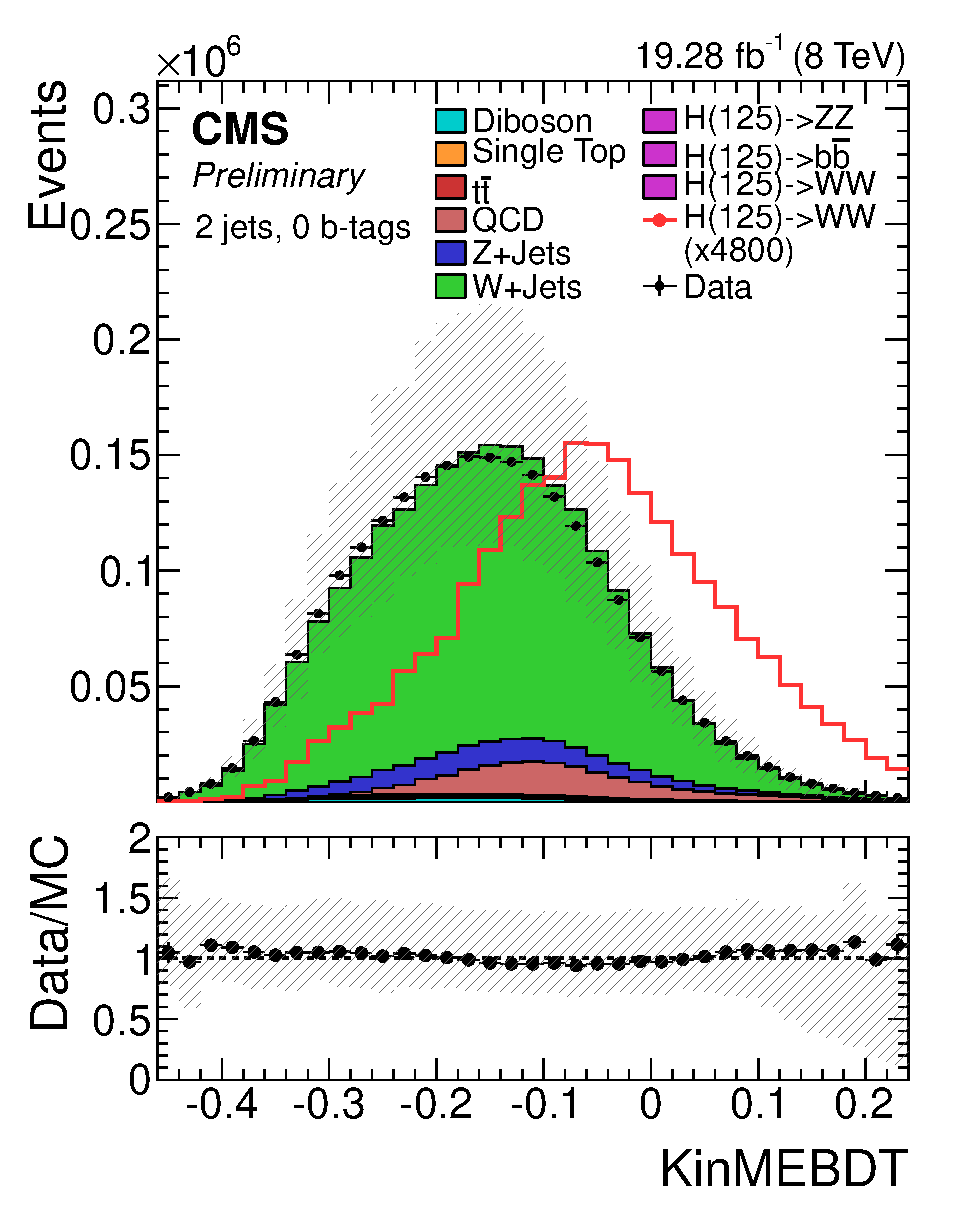
\includegraphics[width=0.26\textwidth]{\figpath/KinMEBDT_jets2_muon.eps}%
    		   \hspace*{0.15cm}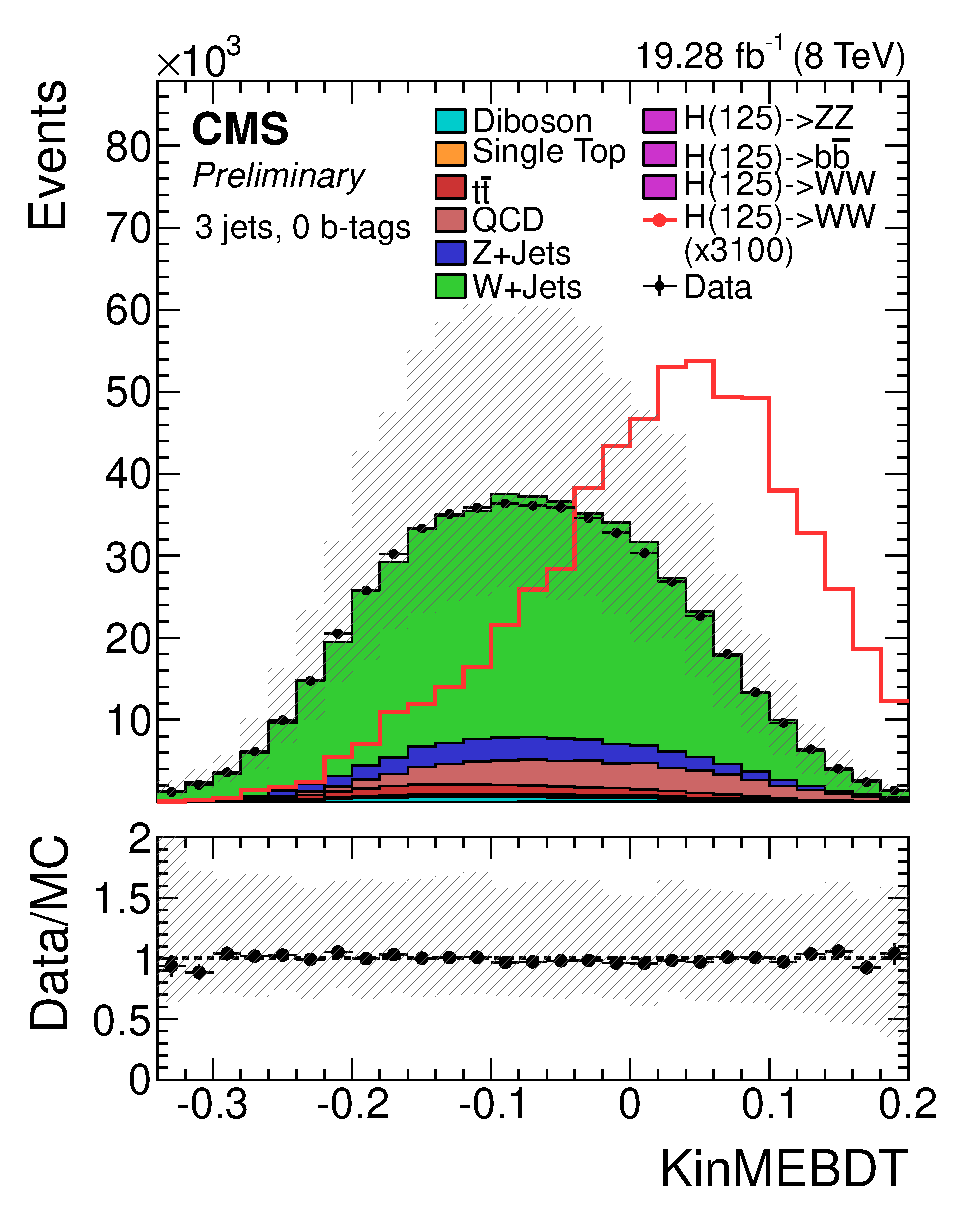
\includegraphics[width=0.26\textwidth]{\figpath/KinMEBDT_jets3_muon.eps}%
    		   \hspace*{0.15cm}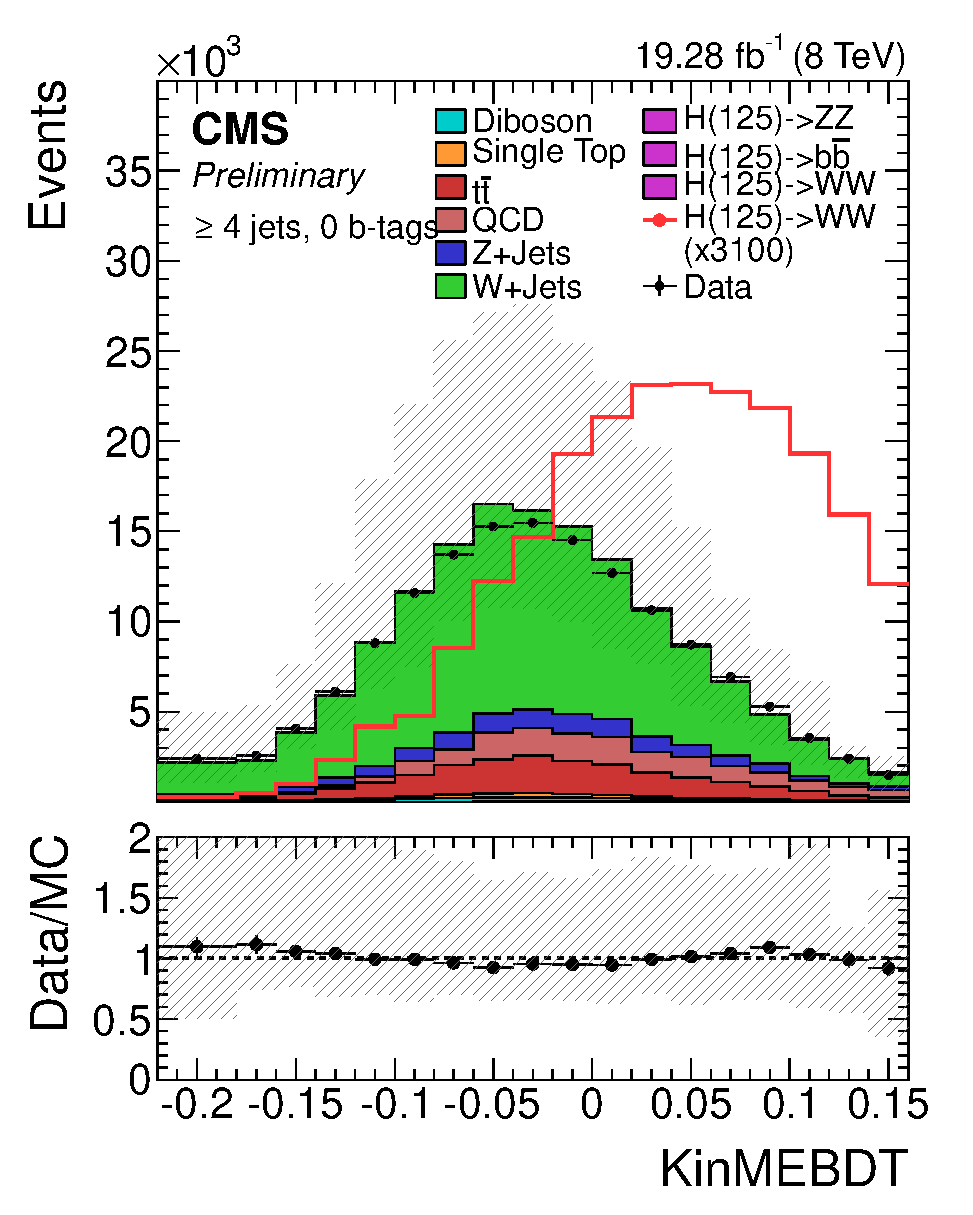
\includegraphics[width=0.26\textwidth]{\figpath/KinMEBDT_jets4_muon.eps}%
    		};

    		\node [draw,rectangle,text centered, rounded corners,fill=tamugray,tamugray,text=Black,rotate=90, left of = image, xshift=1.1cm, yshift=5.5cm] {Electron};
    		\node [draw,rectangle,text centered, rounded corners,fill=tamugray,tamugray,text=Black,rotate=90, left of = image2, xshift=1.1cm, yshift=5.5cm] {Muon};
  		\end{myfancyblock}
  		\begin{textblock}{0.25}(0.225,0.52){\color{red}{2 Jets}}\end{textblock}
  		\begin{textblock}{0.25}(0.49,0.52){\color{red}{3 Jets}}\end{textblock}
  		\begin{textblock}{0.25}(0.74,0.52){\color{red}{$\geqslant$4 Jets}}\end{textblock}
	%\end{alertblock}
\end{frame}

\begin{frame}
	\frametitle{Results}
	\vspace*{-0.24cm}
	\begin{columns}[T]
		\begin{column}{0.6\textwidth}
			\vspace*{-0.6cm}
			\begin{table}[htbp]
				\color{black}
				\caption*{\scriptsize Observed and median expected and 95\% CLs upper limits on $\mu$ calculated with the Asymptotic CL\textsubscript{S} method. The $\pm1\sigma$ confidence interval is quoted for the expected limits.}
				\label{tab:95percent_upper_confidence_levels}
				\centering
				\scriptsize
				\vspace*{-0.15cm}
				\begin{tabular}{|l|r|r|} \hline
					\textbf{Category}                   & \textbf{Observed} & \textbf{Expected} \\
					\hline\\[-2.55ex]
					$\geqslant$4 Jets (\Pe)             & $88.0$   & $50.5_{-13.8}^{+17.1}$ \\
					3 Jets (\Pe)                        & $20.6$   & $18.9_{-5.3}^{+7.5}$   \\
					2 Jets (\Pe)                        & $7.0$    & $7.4_{-2.1}^{+3.0}$    \\
					$\geqslant$4 Jets (\Pmu)            & $19.4$   & $12.6_{-3.5}^{+5.0}$   \\
					3 Jets (\Pmu)                       & $8.0$    & $9.3_{-2.6}^{+3.7}$    \\
					2 Jets (\Pmu)                       & $11.2$   & $8.8_{-2.5}^{+3.6}$    \\
					\hline\\[-2.55ex]
					Combined                            & $5.4$   & $3.4_{-0.9}^{+1.4}$     \\
					\hline
				\end{tabular}
			\end{table}
			\vspace*{-0.2cm}
			\begin{table}[htbp]
				\color{black}
				\label{tab:significances_and_pvalues}
				\caption*{\scriptsize Expected and observed statistical significances as well as their associated p-values. The a-priori expected significances are computed before the background fits to the data. For the two and three jet muon bins the significance is zero because the minimum of the likelihood is for a signal strength $\leqslant0$.}
				\centering
				\tiny
				\vspace*{-0.15cm}
				\begin{tabular}{lrrr} \hline
					Category                            & A-priori Expected & A-posteriori Expected & Observed \\
					\hline\\[-2.45ex]
					$\geqslant$4 Jets (\Pe)             & $0.045$ ($0.482$) & $0.011$ ($0.496$) & $2.647$ ($0.004$) \\
					3 Jets (\Pe)                        & $0.104$ ($0.459$) & $0.096$ ($0.462$) & $2.014$ ($0.022$) \\
					2 Jets (\Pe)                        & $0.178$ ($0.430$) & $0.191$ ($0.424$) & $0.531$ ($0.298$) \\
					$\geqslant$4 Jets (\Pmu)            & $0.192$ ($0.424$) & $0.153$ ($0.439$) & $1.190$ ($0.117$) \\
					3 Jets (\Pmu)                       & $0.218$ ($0.414$) & $0.207$ ($0.418$) & $0.000$ ($0.500$) \\
					2 Jets (\Pmu)                       & $0.208$ ($0.418$) & $0.195$ ($0.423$) & $0.000$ ($0.500$) \\
					\hline\\[-2.45ex]
					Combined                            & $0.569$ ($0.268$) & $0.547$ ($0.292$) & $0.903$ ($0.183$) \\
					\hline
				\end{tabular}
			\end{table}
		\end{column}
		\begin{column}{0.4\textwidth}
			\centering
			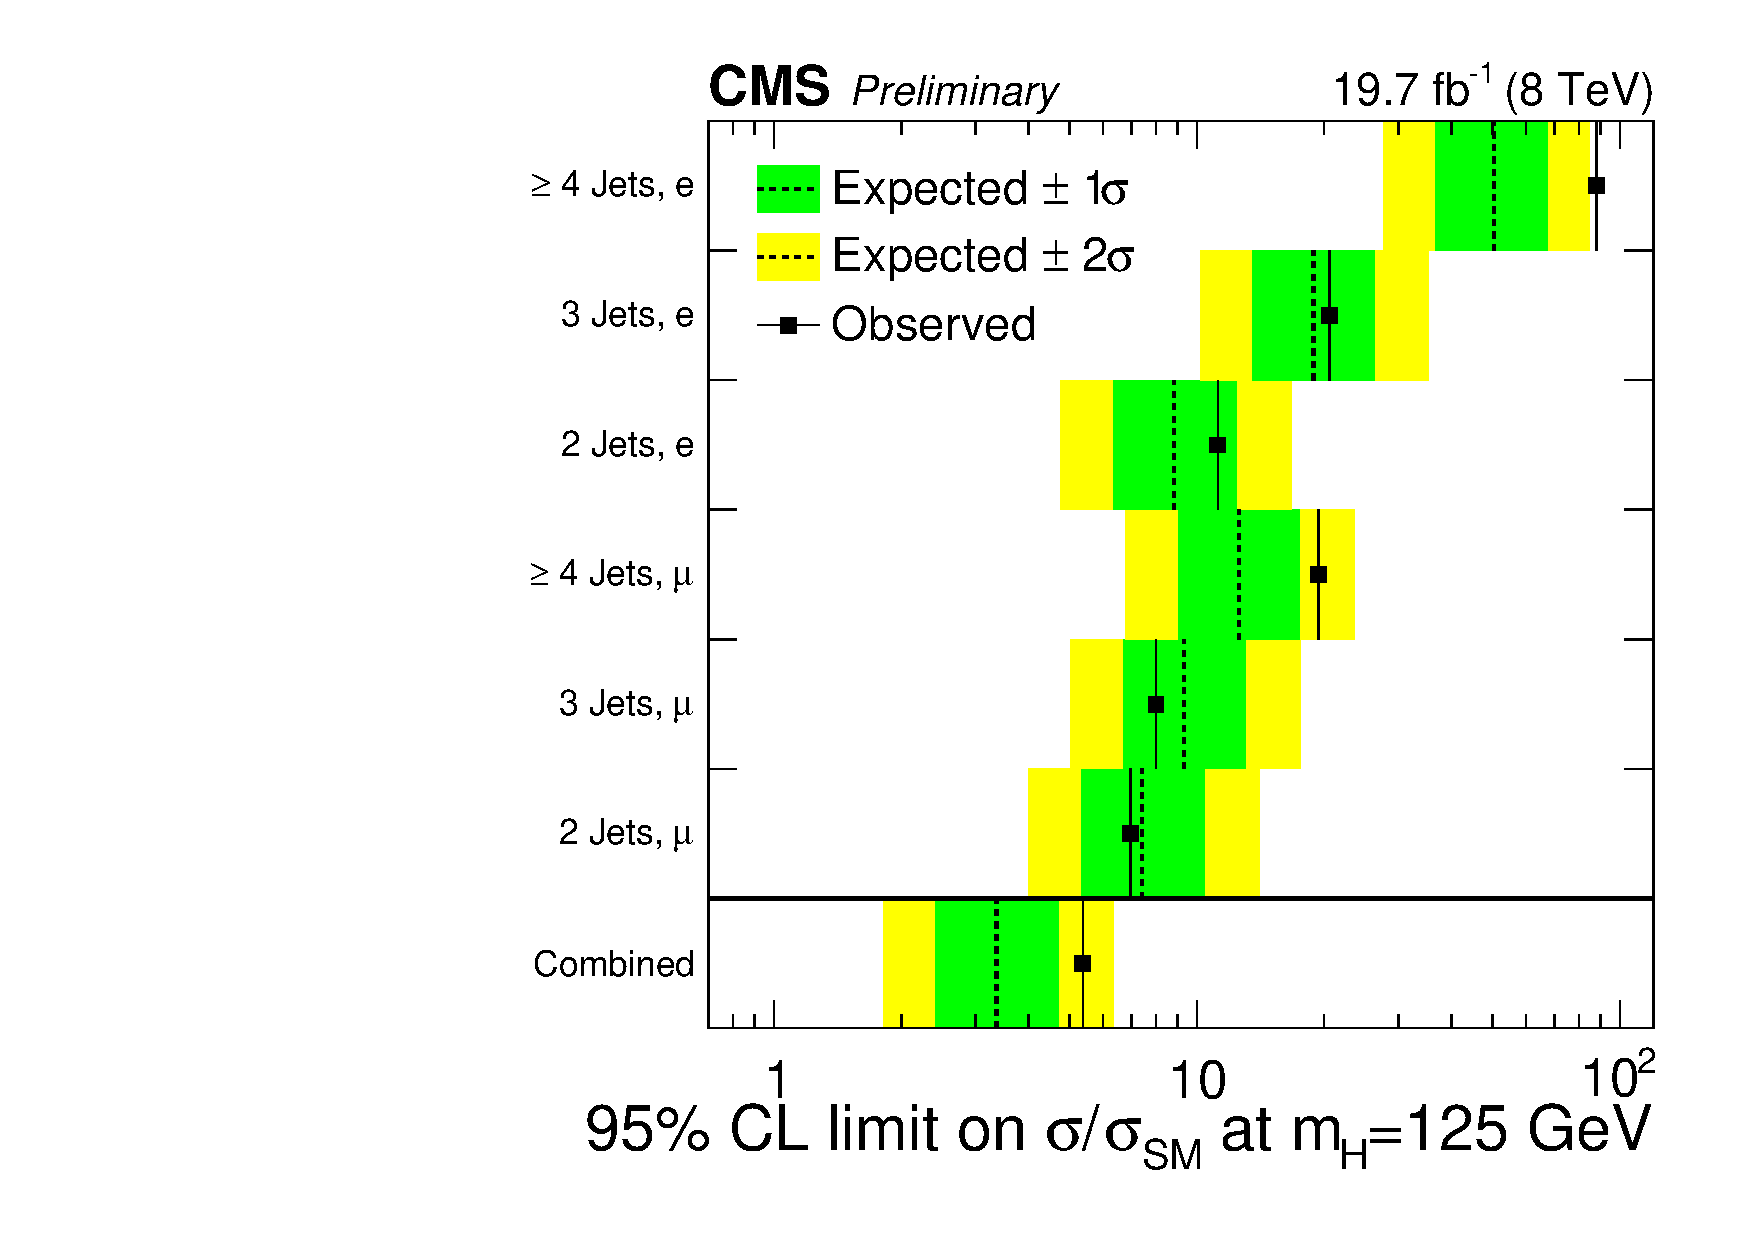
\includegraphics[width=0.85\textwidth]{\figpath/2017_11_15_combinedSM_KinMEBDT.pdf}\\[0.2em]
			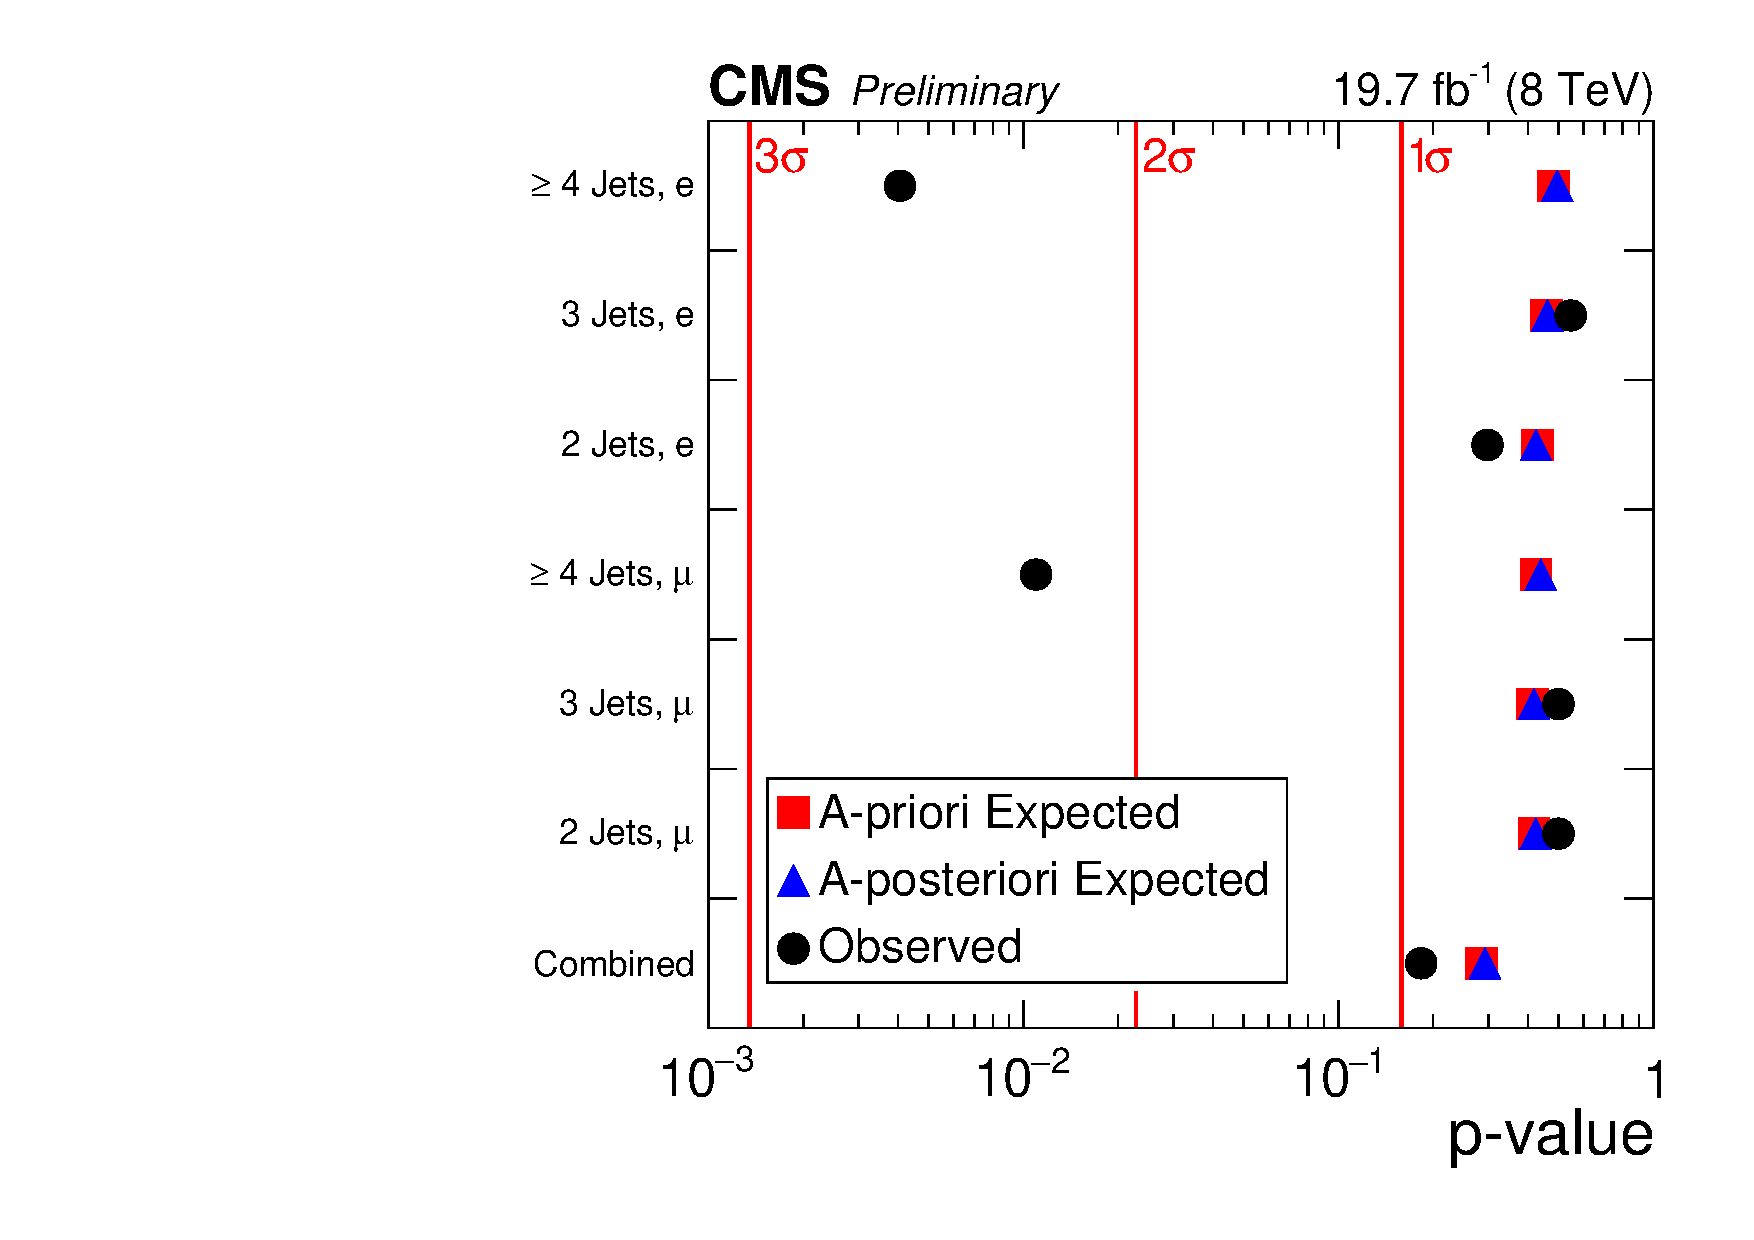
\includegraphics[width=0.85\textwidth]{\figpath/2017_11_15_pvalue_KinMEBDT.pdf}
		\end{column}
	\end{columns}
\end{frame}